\chapter{QR factorization}

\section{projector}

\begin{definition}
    我们称一个 operator $P: \mathbb{C}^n \rightarrow \mathbb{C}^n$ 为一个 projector, if \[
    P^2  = P
    \]
Note: \textbf{不要求是 linear 的.} For linear case, 这是一个\textbf{ idempotent linear map.}
(而我们将主要关注于 linear orthogonal projector.)
\end{definition}
\begin{remark}
一个 projector 总有: \[
P^m = P
\]
对于任意 $m$ 次 composition.\\
即: 在第一次作用后, 之后再对其结果进行这一映射不作出任何改变. \\
直观: 这个映射的效果是把一个向量投影到一个低维度子空间上, 从而, 在作用过一次后, 再次施加这一映射将没有任何改变.\\


\end{remark}

\begin{remark}
    对于 orthogonal 的 projector, 我们称其为 orthogonal projector; 对于 non-orthogonal 的 projector, 我们称其为 oblique projector.\\
    
\end{remark}


\begin{remark}
    projector 虽然不保证是 linear 的, 但是要么是 linear 的, 要么就是个 affine transformation. 和 linear 也差不多. 不用在意这些细节. 
\end{remark}

以下, 我们都只考虑 projector linear 的情况. nonlinear 的情况是类似的.

\begin{lemma}
我们发现, 一个 projector $P$ 沿着 $S_1 := \ker(P)$ 把空间投影到 $S_2 :=im(P)$ 上.
\end{lemma}

\begin{lemma}
    一个 projector 的 eigenvalue 只有可能是 $0$ 或者 $1$. 它的 SVD 同时也是 eigenvalue decomposition: \[
    P = Q \Sigma Q^*
    \]
    其中 $\Sigma$ 是一个前面全 1, 后面全 0 的对角矩阵.
\end{lemma}


\begin{lemma}{complement projector}
    如果 $P$ 是一个 projector, 那么 $I-P$ 也是一个 projector.\\
    我们称 $I-P$ 为 $P$ 的 complementary projector.\\
    并且我们有: \textbf{complementary projector 的 ker 是原 projector 的 im, im 是原 projector 的 ker.}
\end{lemma}

\begin{remark}
    $P$ 把 vectors 沿着 $S_1$ 投影到 $S_2$; \\
    $I - P$ 把 vectors 沿着 $S_2$ 投影到 $S_1$.
\end{remark}


\begin{definition}{orthogonal projector}
    我们称一个 projector 是 orthogonal projector, 如果 $\ker(P) \bot im(P)$.
\end{definition}

\begin{theorem}
    一个 projector $P$ 是 orthogonal projector $\Longleftrightarrow$ $P = P^*$, 即 $P$ 是 Hermitian 的.
\end{theorem}

\begin{theorem}
    一个 projector $P$ 是 orthogonal projector, 则它的 \textbf{complementary projector $I-P$ 也是 orthogonal projector.}
\end{theorem}

\begin{corollary}
    orthogonal projector $P$ 的 complementary $I-P$ 把 vectors 投影到 $im(P)^{\bot}$ 上. 
\end{corollary}

\section{classical Gram-Schmidt orthogonalization}
classical Gram-Schmidt 是计算 reduced QR 分解的算法.
\begin{figure}
    \centering
    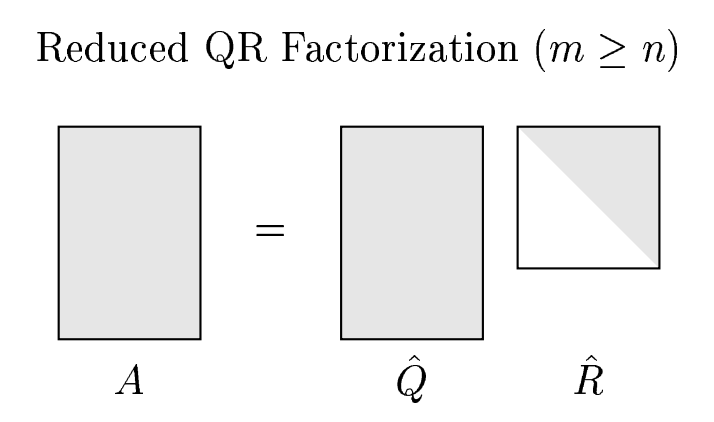
\includegraphics[width=0.5\linewidth]{assets/Screenshot 2025-04-17 at 11.44.46.png}
    \caption{reduced QR}
    \label{fig:reduced QR}
\end{figure}
\subsection{idea of triangular orthogonalization}
classical Gram-Schmidt orthogonalization 的 idea 是: 我们逐列地将 $A$ 的 columns 转变为相互 orthogonal 的新列.\\
具体: 我们每次都把 $a_j$ 减去 $a_1,\cdots, a_{j-1}$ 的 span 包含的成分, 从而制作成和  $a_1,\cdots, a_{j-1}$ 的 span 正交的新列 $q_j$: 
\begin{align*}
q_j := \text{normalized} (& \,a_j - \text{proj}_ {\langle a_1,\cdots,a_{j-1} \rangle} a_j) \\
=  \text{normalized} (& \,a_j- \text{proj}_ {\langle q_1,\cdots,q_{j-1} \rangle} a_j)
\end{align*}
展开这个定义: 
\begin{align*}
v_j&:=a_j-\left(q_1^* a_j\right) q_1-\left(q_2^* a_j\right) q_2-\cdots-\left(q_{j-1}^* a_j\right) q_{j-1}\\
    q_j  &:= v_j / |v_j|  
\end{align*}
这个过程可以通过定义: 
$$
r_{i j}=q_i^* a_j \;(i \neq j), \quad   \left|r_{j j}\right|=\left\|a_j-\sum_{i=1}^{j-1} r_{i j} q_i\right\|_2
$$
(Note that the sign of $r_{j j}$ is not determined. Arbitrarily, we may choose $r_{j j}>0$, in which case we shall finish with a factorization $A=\hat{Q} \hat{R}$ in which $\hat{R}$ has positive entries along the diagonal.)\\
从而这个过程写作: 
\begin{align*}
v_j &:=a_j -  \sum_{i=1}^{j-1} r_{i j} q_i    \\
q_j  &:= v_j / r_{jj}  
\end{align*}
我们发现:
$$
\begin{aligned}
q_1 & =\frac{a_1}{r_{11}} \\
q_2 & =\frac{a_2-r_{12} q_1}{r_{22}}, \\
q_3 & =\frac{a_3-r_{13} q_1-r_{23} q_2}{r_{33}}, \\
& \vdots \\
q_n & =\frac{a_n-\sum_{i=1}^{n-1} r_{i n} q_i}{r_{n n}}
\end{aligned}
$$
这个过程使得: 
\[
a_j = \sum_{i=1}^j r_{ij} q_i
\]从而:
\[
A  = \hat{Q} \hat{R}
\]

\subsection{algorithm}


\begin{algorithm}
\caption{Classical Gram-Schmidt (unstable)}
\begin{algorithmic}[1]
\FOR{$j = 1$ \TO $n$}
    \STATE $v_j \gets a_j$
    \FOR{$i = 1$ \TO $j-1$}
        \STATE $r_{ij} \gets q_i^* a_j$
        \STATE $v_j \gets v_j - r_{ij} q_i$
    \ENDFOR
    \STATE $r_{jj} \gets \|v_j\|_2$
    \STATE $q_j \gets v_j / r_{jj}$
\ENDFOR
\end{algorithmic}
\end{algorithm}




\section{modified Gram-Shimitdt (triangular orthogonalization)}





\section{Household Triangularization}






